\section{Aufgabe 3} \label{ex3}

Konfiguration des IP Cores zur Realisierung der Kommunikation zwischen Prozessor und 
Peripherie als Blockdesign in Vivado 2016.2. Eingebunden in diese wurden zusätzlich die 8Bit-LED-Anzeige und die Push-Buttons. Der Aufbau wurde anschließend in VHDL synthetisiert. 

\begin{minipage}{\textwidth}
    \begin{center}        
        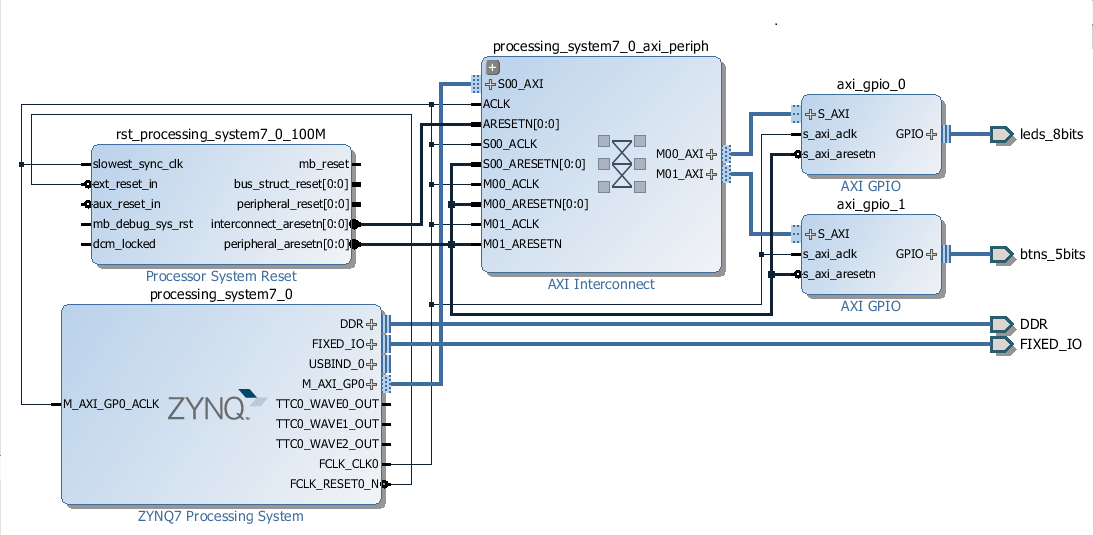
\includegraphics[scale=0.6]{img/a3.png} 
    \end{center}
\end{minipage}
\begin{center}
Vivado: Schemaplan der IP-Cores
\end{center}

Programmcode zur Abfrage der Buttons and Zuweisung des Bit-Musters direkt an die LEDs.
\begin{verbatim}
#include  <stdio.h>
#include "platform.h"
#include "xparameters.h"
#include "xgpio.h"
#include "xstatus.h"
#include "xil_printf.h"
//  Definitions
#define  LEDS_DEVICE_ID  XPAR_AXI_GPIO_0_DEVICE_ID
#define  BTNS_DEVICE_ID  XPAR_AXI_GPIO_1_DEVICE_ID

#define  LED_DELAY  1000000
#define  LED_CHANNEL 1
#define  printf  xil_printf

XGpio  Gpio;
XGpio LEDInst , BTNInst ;
static int btn_value ;

int  LEDOutputExample( VOID ) {
	volatile  int  Delay;
	// loop  forever  blinking  the  LED.
	while( 1 ) {
		// read buttons
		btn_value = XGpio_DiscreteRead (&BTNInst , 1);
		//  write  button value  to LEDs
		XGpio_DiscreteWrite( &LEDInst , LED_CHANNEL , btn_value );

		for ( Delay = 0;  Delay  < LED_DELAY; Delay++ );
	}
	return  XST_SUCCESS;
}

int  main()
{
	init_platform ();

	int status ;
	// ----------------------------------------------------
	// INITIALIZE THE PERIPHERALS & SET DIRECTIONS OF GPIO
	// ----------------------------------------------------
	// Initialise LEDs
	status = XGpio_Initialize (&LEDInst , LEDS_DEVICE_ID );
	if ( status != XST_SUCCESS )
		return XST_FAILURE ;

	// Initialise Push Buttons
	status = XGpio_Initialize (&BTNInst , BTNS_DEVICE_ID );
	if ( status != XST_SUCCESS )
		return XST_FAILURE ;

	// Set LEDs direction to outputs
	XGpio_SetDataDirection (&LEDInst,1,0x00);
	// Set all buttons direction to inputs
	XGpio_SetDataDirection (&BTNInst,1,0xFF);

	print("Hello  meine  LED\n\r");

	LEDOutputExample ();
	cleanup_platform ();
	return  0;
}
\end{verbatim}

\begin{minipage}{\textwidth}
    \begin{center}        
        
\includegraphics[scale=0.6]{img/button.png} 
    \end{center}
\end{minipage}
\begin{center}
Zuordnung der Buttons
\end{center}

Das zugehörige Bitmuster pro Button ist:\\
Button1 BTNU: 0001 0000b, 0x10\\
Button2 BTNL: 0000 0100b, 0x04\\
Button3 BTNC: 0000 0001b, 0x01\\
Button4 BTNR: 0000 1000b, 0x08\\
Button5 BTNO: 0000 0010b, 0x02\\
